\documentclass[11pt, a4paper]{article}
\usepackage[utf8]{inputenc}
\usepackage{times}
\usepackage[left=2cm, top=3cm, text={17cm,24cm}]{geometry}
\usepackage[czech]{babel}
\usepackage[IL2]{fontenc}
\usepackage[hidelinks]{hyperref}
\usepackage{multirow}
\usepackage{multicol}
\usepackage[linesnumbered, ruled, noline, longend]{algorithm2e}
\usepackage{graphics}
\usepackage{picture}

\renewcommand\UrlFont{}
\renewcommand{\algorithmcfname}{Algoritmus}

\begin{document}

\catcode`\-=12 % fix pro cline

\begin{titlepage}
\begin{center}
    \Huge
    \textsc{Vysoké učení technické v Brně}\\
    \huge
    \textsc{Fakulta informačních technologií}\\
    \vspace{\stretch{0.382}}
    \LARGE
    Typografie a publikování -- 3. projekt\\
    \Huge
    Tabulky a obrázky
    \vspace{\stretch{0.618}}
\end{center}
{\Large \today \hfill Jakub Hlava}
\end{titlepage}
\newpage

\section{Úvodní strana}
Název práce umístěte do zlatého řezu a nezapomeňte uvést dnešní datum a vaše jméno a příjmení.
\section{Tabulky}
Pro sázení tabulek můžeme použít buď prostředí \texttt{tabbing} nebo prostředí \texttt{tabular}.
\subsection{Prostředí \texttt{tabbing}}
Při použití \texttt{tabbing} vypadá tabulka následovně:
\begin{tabbing}
Vodní melouny\quad \= 25,90\quad \= \kill
\textbf{Ovoce} \> \textbf{Cena} \>  \textbf{Množství} \\
Jablka \>  25,90 \> 3 kg \\
Hrušky \>  27,40 \>  2,5 kg \\
Vodní melouny \>  35,-- \>  1 kus
\end{tabbing}
\vspace{1em}
Toto prostředí se dá také použít pro sázení algoritmů, ovšem vhodnější je použít 
prostředí algorithm nebo algorithm2e (viz sekce 3). % doplnit křížový odkaz
\subsection{Prostředí \texttt{tabular}}
Další možností, jak vytvořit tabulku, je použít prostředí \texttt{tabular}. Tabulky pak 
budou vypadat takto \footnote{Kdyby byl problem s \texttt{cline}, zkuste se podívat třeba sem: \url{http://www.abclinuxu.cz/tex/poradna/show/325037}}:
\vspace{1em}
\begin{table}[h]
    \centering
    \begin{tabular}{|c|c|c|}
        \hline
         & \multicolumn{2}{|c|}{\textbf{Cena}} \\ \cline{2-3}
        \textbf{Měna} & \textbf{nákup} & \textbf{prodej} \\ \hline
         EUR & 25,475 & 27,045 \\ 
         GBP & 28,835 & 30,705 \\
         USD & 22,943 & 24,357 \\ \hline
    \end{tabular}\\
    \caption{Tabulka kurzů k dnešnímu dni}\label{tab-meny}
\end{table}
\vspace{1em}
\begin{table}[h]
    \centering
    \begin{tabular}{|c|c|}
        \hline
        A & $\neg$A \\ \hline
        \textbf{P} & N \\ \hline
        \textbf{O} & O \\ \hline
        \textbf{X} & X \\ \hline
        \textbf{N} & P \\ \hline
    \end{tabular}
    \begin{tabular}{|c|c|c|c|c|c|}
        \hline
        \multicolumn{2}{|c|}{\multirow{2}{*}{A $\wedge$ B}} & \multicolumn{4}{|c|}{B} \\ \cline{3-6}
        \multicolumn{2}{|c|}{} & \textbf{P} & \textbf{O} & \textbf{X} & \textbf{N} \\ \hline
        \multirow{4}{1em}{A} & \textbf{P} & P & O & X & N \\ \cline{2-6}
         & \textbf{O} & O & O & N & N \\ \cline{2-6}
         & \textbf{X} & X & N & X & N \\ \cline{2-6}
         & \textbf{N} & N & N & N & N \\ \hline
    \end{tabular}
    \begin{tabular}{|c|c|c|c|c|c|}
        \hline
        \multicolumn{2}{|c|}{\multirow{2}{*}{A $\vee$ B}} & \multicolumn{4}{|c|}{B} \\ \cline{3-6}
        \multicolumn{2}{|c|}{} & \textbf{P} & \textbf{O} & \textbf{X} & \textbf{N} \\ \hline
        \multirow{4}{1em}{A} & \textbf{P} & P & P & P & P \\ \cline{2-6}
        & \textbf{O} & P & O & P & O \\ \cline{2-6} 
        & \textbf{X} & P & P & X & X \\ \cline{2-6}
        & \textbf{N} & P &O & X & N \\ \hline
    \end{tabular}
    \begin{tabular}{|c|c|c|c|c|c|}
         \hline
        \multicolumn{2}{|c|}{\multirow{2}{*}{A $\rightarrow$ B}} & \multicolumn{4}{|c|}{B} \\ \cline{3-6}
        \multicolumn{2}{|c|}{} & \textbf{P} & \textbf{O} & \textbf{X} & \textbf{N} \\ \hline
        \multirow{4}{1em}{A} & \textbf{P} & P & O & X & N \\ \cline{2-6}
        & \textbf{O} & P & O & P & O \\ \cline{2-6} 
        & \textbf{X} & P & P & X & X \\ \cline{2-6}
        & \textbf{N} & P & P & P & P \\ \hline
    \end{tabular}
    \caption{Protože Kleeneho trojhodnotová logika už je \uv{zastaralá}, uvádíme si zde příklad čtyřhodnotové logiky}\label{tab-fce}
\end{table}
\newpage
\section{Algoritmy}
Pokud budeme chtít vysázet algoritmus, můžeme použít prostředí \texttt{algorithm}\footnote{Pro nápovědu, jak zacházet s prostředím \texttt{algorithm}, můžeme zkusit tuhle stránku:\\
\url{http://ftp.cstug.cz/pub/tex/CTAN/macros/latex/contrib/algorithms/algorithms.pdf}.} nebo \texttt{algorithm2e}\footnote{Pro \texttt{algorithm2e} zase tuhle:
\url{http://ftp.cstug.cz/pub/tex/CTAN/macros/latex/contrib/algorithm2e/algorithm2e.pdf}.}.
Příklad použití prostředí \texttt{algorithm2e} viz Algoritmus 1. % doplnit křížový odkaz
\\[2em]
\begin{algorithm}[H]
\label{algo-fastslam}
\caption{\textsc{FastSLAM}}
    \DontPrintSemicolon
    \SetKwInput{KwInput}{Input}
    \SetKwInput{KwOutput}{Output}
    \KwInput{$(X_t-1, u_t, z_t)$}
    \KwOutput{$X_t$}
    \BlankLine
    $\overline{X_t} = X_t = 0$\;
    \For{$k = 1$ to $M$}{
        $x_t^{[k]} =\ $\emph{sample\_motion\_model}$(u_t, x_{t-1}^{[k]})$\;
        $\omega_t^{[k]} =\ $\emph{measurement\_model}$(z_t, x_t^{[k]})$\;
        $m_t^{[k]} =\ $\emph{updated\_occupancy\_grid}$(z_t,x_t^{[k]},m_{t-1}^{[k]})$\;
        $\overline{X_t} = \overline{X_t} + \left<x_x^{[m]}, \omega_t^{[m]} \right>$\;
    }
    \For{$k = 1$ \emph{to} $M$}{
        draw $i$ with probability $\approx \omega_t^{[i]}$\;
        add $\left< x_x^{[k]}, m_t^{[k]} \right>$ to $X_t$\;
    }
    \Return{$X_t$}
\end{algorithm}

\section{Obrázky}
Do našich článků můžeme samozřejmě vkládat obrázky. Pokud je obrázkem fotografie,
můžeme klidně použít bitmapový soubor. Pokud by to ale mělo být nějaké schéma nebo
něco podobného, je dobrým zvykem takovýto obrázek vytvořit vektorově.
\par
\begin{figure}[h]
\centering
    \scalebox{0.4}{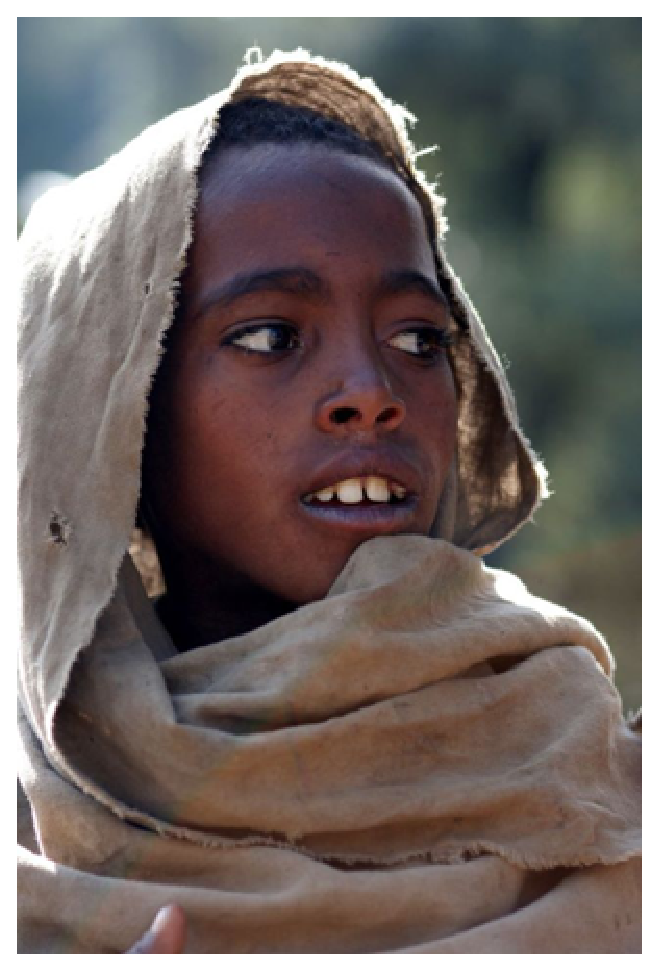
\includegraphics{img/etiopan.eps}
\reflectbox{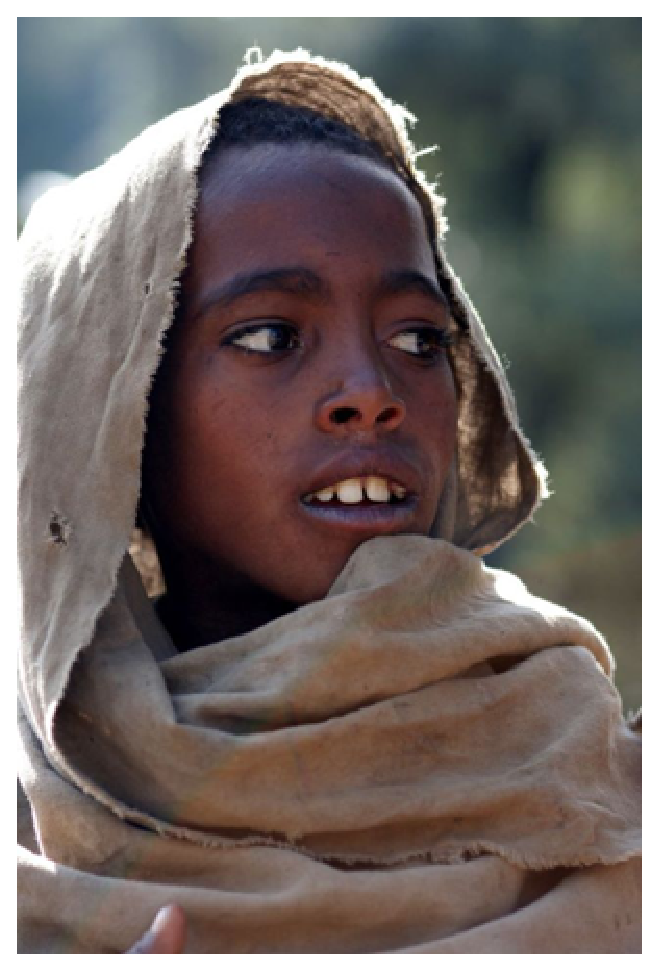
\includegraphics{img/etiopan.eps}}}
\caption{Malý Etiopánek a jeho bratříček}\label{img-etiopani}
\end{figure}
\newpage
Rozdíl mezi vektorovým \ldots \\
\begin{figure}[h]
\centering
\scalebox{0.5}{
\includegraphics{img/oniisan.eps}}
\caption{Vektorový obrázek}\label{img-vektor}
\end{figure} \\
\ldots a bitmapovým obrázkem \\
\begin{figure}[h]
\centering
\scalebox{0.7}{
\includegraphics{img/oniisan2.eps}}
\caption{Bitmapový obrázek}\label{img-bitmap}
\end{figure} \\
se projeví například při zvětšení.
\par
Odkazy (nejen ty) na obrázky \ref{img-etiopani}, \ref{img-vektor} a \ref{img-bitmap}, na  
tabulky \ref{tab-meny} a \ref{tab-fce} a také na algoritmus \ref{algo-fastslam} jsou udělány pomocí 
křížových odkazů. Pak je ovšem potřeba zdrojový soubor přeložit dvakrát.
\par
Vektorové obrázky lze vytvořit i přímo v \LaTeX{}u, například pomocí prostředí 
\texttt{picture}.
\newpage
\begin{figure}[h]
\centering
\begin{picture}(450, 350)
%slunicko
\put(400,300){\circle{30}}
\put(400,330){\line(0,1){20}}
\put(400,275){\line(0,-1){16}}
\put(375,300){\line(-1,0){25}}
\put(430,300){\line(1,0){12}}
\put(420,320){\line(1,1){10}}
\put(420,280){\line(1,-1){15}}
\put(380,320){\line(-1,1){19}}
\put(380,280){\line(-1,-1){10}}
%obvod+zakladna
\thicklines
\put(430,0){\line(0,1){200}}
\put(20,35){\line(0,1){165}}
\linethickness{2pt}
\put(0,35){\line(1,0){280}}
\put(450,0){\line(-1,0){130}}
\put(320,0){\line(0,1){11}}
\put(300,11){\line(0,1){12}}
\put(280,23){\line(0,1){12}}
\put(320,11){\line(-1,0){20}}
\put(300,23){\line(-1,0){20}}
\thinlines
%vrata
\put(420,0){\line(0,1){100}}
\put(340,0){\line(0,1){100}}
\put(340,100){\line(1,0){80}}
\put(380,0){\line(0,1){100}}

\put(345,95){\line(1,0){30}}
\put(345,80){\line(1,0){30}}
\put(345,80){\line(0,1){15}}
\put(355,80){\line(0,1){15}}
\put(365,80){\line(0,1){15}}
\put(375,80){\line(0,1){15}}
\put(385,95){\line(1,0){30}}
\put(385,80){\line(1,0){30}}
\put(385,80){\line(0,1){15}}
\put(395,80){\line(0,1){15}}
\put(405,80){\line(0,1){15}}
\put(415,80){\line(0,1){15}}
\put(345,60){\framebox(30,15){}}
\put(345,35){\framebox(30,15){}}
\put(345,10){\framebox(30,15){}}
\put(385,60){\framebox(30,15){}}
\put(385,35){\framebox(30,15){}}
\put(385,10){\framebox(30,15){}}

%okno1
\put(50,60){\line(0,1){60}}
\put(50,60){\line(1,0){50}}
\put(100,60){\line(0,1){60}}
\put(50,120){\line(1,0){50}}

\put(53,63){\line(0,1){55}}
\put(97,63){\line(0,1){55}}
\put(73,63){\line(0,1){55}}
\put(77,63){\line(0,1){55}}
\put(53,118){\line(1,0){20}}
\put(77,118){\line(1,0){20}}
\put(53,63){\line(1,0){20}}
\put(77,63){\line(1,0){20}}
%okno2
\put(160,60){\line(0,1){60}}
\put(160,60){\line(1,0){50}}
\put(210,60){\line(0,1){60}}
\put(160,120){\line(1,0){50}}

\put(163,63){\line(0,1){55}}
\put(207,63){\line(0,1){55}}
\put(183,63){\line(0,1){55}}
\put(187,63){\line(0,1){55}}
\put(163,118){\line(1,0){20}}
\put(187,118){\line(1,0){20}}
\put(163,63){\line(1,0){20}}
\put(187,63){\line(1,0){20}}
%okno3
\put(270,60){\line(0,1){60}}
\put(270,60){\line(1,0){50}}
\put(320,60){\line(0,1){60}}
\put(270,120){\line(1,0){50}}

\put(273,63){\line(0,1){55}}
\put(317,63){\line(0,1){55}}
\put(293,63){\line(0,1){55}}
\put(297,63){\line(0,1){55}}
\put(273,118){\line(1,0){20}}
\put(297,118){\line(1,0){20}}
\put(273,63){\line(1,0){20}}
\put(297,63){\line(1,0){20}}
%horniokna
%okno1
\put(50,150){\line(0,1){40}}
\put(50,150){\line(1,0){50}}
\put(100,150){\line(0,1){40}}
\put(50,190){\line(1,0){50}}

\put(53,153){\line(1,0){12}}
\put(69,153){\line(1,0){12}}
\put(85,153){\line(1,0){12}}
\put(53,187){\line(1,0){12}}
\put(69,187){\line(1,0){12}}
\put(85,187){\line(1,0){12}}

\put(53,153){\line(0,1){34}}
\put(65,153){\line(0,1){34}}
\put(69,153){\line(0,1){34}}
\put(81,153){\line(0,1){34}}
\put(85,153){\line(0,1){34}}
\put(97,153){\line(0,1){34}}
%okno2
\put(160,150){\line(0,1){40}}
\put(160,150){\line(1,0){50}}
\put(210,150){\line(0,1){40}}
\put(160,190){\line(1,0){50}}

\put(163,153){\line(1,0){12}}
\put(179,153){\line(1,0){12}}
\put(195,153){\line(1,0){12}}
\put(163,187){\line(1,0){12}}
\put(179,187){\line(1,0){12}}
\put(195,187){\line(1,0){12}}

\put(163,153){\line(0,1){34}}
\put(175,153){\line(0,1){34}}
\put(179,153){\line(0,1){34}}
\put(191,153){\line(0,1){34}}
\put(195,153){\line(0,1){34}}
\put(207,153){\line(0,1){34}}
%okno3
\put(270,150){\line(0,1){40}}
\put(270,150){\line(1,0){50}}
\put(320,150){\line(0,1){40}}
\put(270,190){\line(1,0){50}}

\put(273,153){\line(1,0){12}}
\put(289,153){\line(1,0){12}}
\put(305,153){\line(1,0){12}}
\put(273,187){\line(1,0){12}}
\put(289,187){\line(1,0){12}}
\put(305,187){\line(1,0){12}}

\put(273,153){\line(0,1){34}}
\put(285,153){\line(0,1){34}}
\put(289,153){\line(0,1){34}}
\put(301,153){\line(0,1){34}}
\put(305,153){\line(0,1){34}}
\put(317,153){\line(0,1){34}}
%okno4
\put(355,150){\line(0,1){40}}
\put(355,150){\line(1,0){50}}
\put(405,150){\line(0,1){40}}
\put(355,190){\line(1,0){50}}

\put(358,153){\line(1,0){12}}
\put(374,153){\line(1,0){12}}
\put(390,153){\line(1,0){12}}
\put(358,187){\line(1,0){12}}
\put(374,187){\line(1,0){12}}
\put(390,187){\line(1,0){12}}

\put(358,153){\line(0,1){34}}
\put(370,153){\line(0,1){34}}
\put(374,153){\line(0,1){34}}
\put(386,153){\line(0,1){34}}
\put(390,153){\line(0,1){34}}
\put(402,153){\line(0,1){34}}
%strecha
\thicklines
\put(10,200){\line(1,0){430}}
\put(10,200){\line(2,1){60}}
\put(440,200){\line(-2,1){60}}
\put(70,230){\line(1,0){310}}
\end{picture}
\caption{Vektorový obrázek mého domu stojícího v kopci}
\end{figure}


\end{document}
